\chapter{Overview of the Theory of HYPERION}

\section{Absorber -- A New Approach to Monopole Interferometry}

If you were to wander onto almost any given radio telescope currently active in 
taking observations, you're almost certain to find some kind of reflective 
material underneath the antennas (either in the form of a ground screen or a 
reflective dish). One thing you're not likely to find is any kind of absorptive 
material -- we as astronomers are already fighting an uphill battle on 
attaining the very fine sensitivities needed to detect celestial sources, we 
really need all the photons we can get. 

However, it is not unheard of. While absorbers have never been used in the 
element design of a reionization project to date, they have been used by cosmic 
microwave background (CMB) experiments. Absorptive structures, or baffles, to 
control pickup from outside the main beam, which can be a source of systemic 
errors~\citet{essinger-hileman2016}. By surrounding the receiver with an 
absorptive material, rather an a reflective one as seen in most standard radio 
telescope designs, one can better control the exact signal that will be seen in 
the sidelobes of the beam, and thereby better calibrate the system in turn.

This same principle applies in the case of a monopole interferometer, where use 
of an absorber can not only be beneficial but actually fundamental to the 
design of the array despite the microscopic signal we aim to detect. By 
controlling what each antenna sees on the sky, we can accurately calibrate our 
system and ensure that our reionization signal is indeed signal and not 
instrumental noise. 

\subsection{Practical Instrumentation}

As discussed in Chapter~\ref{chap:interferometry}, one of the fundamental 
requirements of a monopole interferometer is close spacing of the antennas, in 
order to maximize reception of the global sky mode. However, this close spacing 
also predisposes the instrument to cross-talk. As discussed 
in~\citet{venumadhav2016}, this isn't necessarily a bad thing -- cross-talk is 
one of two ways that an array of antennas can maintain a sensitivity to the 
monopole. Each individual antenna will broadcast its reception of the monopole 
to its neighbors, and that reception will correlate. In this case, one will 
have a direct view of the monopole term, as you will be correlating the 
zero-spacing mode seen by one antenna with the zero-spacing mode of another, 
thus providing the necessary sensitivity to the global signal. 

However, that also means that instrumental noise will be broadcast and 
correlated between antennas, vastly diminishing the useful properties of the 
interferometer and maintaining many of the pitfalls of single-dish instruments.  
The risk here comes in the calculus of calibration for the instrument.
In particular, it is difficult to properly calibrate the correlated noise 
between elements as it has a noise bias. This bias means that, while we observe 
more of the true signal, we also no longer are able to integrate down the 
instrumental noise, essentially placing a DC offset into our system. The exact 
value of this offset is a function of frequency and of the exact qualities of 
the instrument, and will likely vary from element to element. If it is not 
perfectly calibrated and subtracted off from the data, then traces of this bias 
will remain in the final data and can easily be mistaken for true science.

So we'd like to avoid cross-talk and other sources of correlated noise between 
elements as best as we can, while still maintaining a sensitivity to a 
correlated monopole signal. The only other way for an interferometer to have 
the capacity to observe the monopole is through the presence of dissipative 
elements, such as absorbers and/or the ground.  Without cross-talk or 
dissipative elements, the monopole term will integrate to zero in every 
non-zero spatial mode, making the interferometer completely insensitive to the 
global signal~\citet{venumadhav2016}.

One way to manage cross-talk it to pack the space between antennas with 
absorber -- with a high-enough quality absorber, we can essentially make the 
antennas invisible to each other by just placing a tall enough wall between 
them.  Ideally, this material would be quite physically thin, so that these 
absorber walls wouldn't force us to spread the shape of the array at all, thus 
maintaining a sensitivity to the spatial monopole of the reionization global 
signal.

In order for this to work, the absorber needs to meet some basic criteria. Most 
importantly, it will need to be at least optically thick enough that antennas 
on opposing sides of an absorber wall will not observe the same noise signal 
from the absorber. If the noise observed from the absorber is coherent between 
elements, then we will fall into the same pitfalls that arise from cross-talk 
between elements, described above.

Additionally, the absorber walls need to be shaped in such a way that signal 
won't reflect and bounce over the barriers -- if signals are able to diffract 
off of one antenna and into the other, then there will still be cross-talk and 
our calibrations will be flawed. For this reason, we won't be able to build 
straight walls with sharp cutoffs. Rather, we want to build our walls in a way 
that signal gets trapped into the absorber or angles out of the array entirely.  
Ideally, we'd like to build our walls with some kind of pyramidal structure (to 
capture and dampen the signal within the absorber), and with a curved roll-off 
at the top edge (to prevent reflections off of the baffle into multiple 
antennas).

\subsection{Manipulating the Spatial Monopole}

Another benefit to the use of absorber in our array is how we can use it to 
manipulate the instrument's sensitivity to the monopole.  As discussed in 
Sec.~\ref{sec:observing-monopole}, by applying a spatial windowing function to 
our monopole signal, we can increase our interferometric sensitivity to the 
global signal. The absorber can impose this windowing function by creating a 
spatial temperature change in the absorber's field of view, increasing the 
harmonic content of the monopole signal by imposing non-isotropic terms.

\begin{figure}
    \begin{center}
    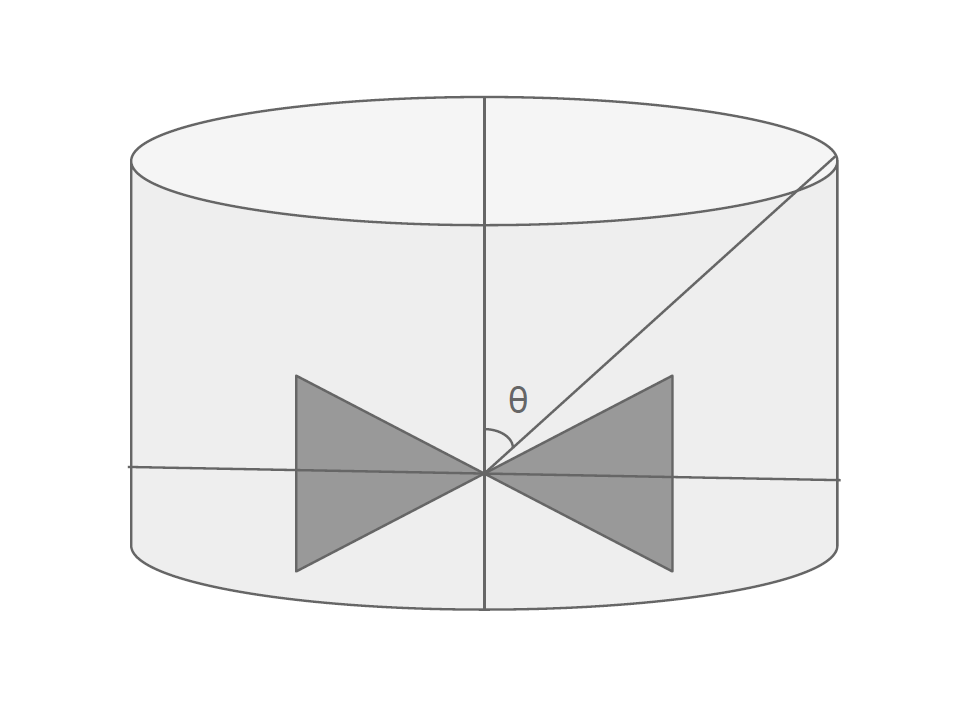
\includegraphics[width=\linewidth]{absorber-structure.png}
    \end{center}
    \caption{
        This cartoon shows the basic structure of the proposed absorber walls.  
        Each antenna in the array will be circled by a cylinder of absorber 
        material, creating a uniform temperature cutoff in the antenna's 
        reception of the sky. By increasing the height of the wall, we can 
        change the cutoff angle of the reception of the sky, thereby shrinking 
        the spatial windowing and pushing more of the monopole to higher 
        spatial modes.
    }
    \label{fig:absorber-structure}
\end{figure}

Let's take a closer look at how this is to actually work. In a perfect world, 
our absorbing material would be $100\%$ effective and no information could be 
transmitted through it -- it would absorb all incident light and re-emit it as 
thermal radiation. That means that, as per Fig.~\ref{fig:absorber-structure} 
and ignoring the effects of the antenna beam shape, the antenna would see the 
sky up until an angle of $\theta$ off of zenith, and then it would see a 
perfect blackbody matching the ambient temperature of the array everywhere 
else.

One way to understand the absorption of the blackbody would be to think in 
terms of optical depth, and the above case is one in which the absorber has an 
optical depth of $\tau = \infty$. This thinking also enables us to begin to 
understand more realistic scenarios, where we don't have perfect absorption 
between our antennas.

\begin{equation}
    I_{obs}(\theta) = I_{sky}~e^{-\tau_\theta} + S_{abs}~(1 - e^{-\tau_\theta})
    \label{eq:abs-optical-depth}
\end{equation}

where $I_{obs}$ is the observed sky brightness, $I_{sky}$ is the sky 
brightness, $S_{abs}$ is the thermal brightness from the absorber, and $\tau$ 
is the optical depth of the absorber. This equation is a variation on the 
radiative transfer equation, where the sky is our source and the absorber is 
the medium through which the radiation is travelling.

In this quantitative construction of the reception of an element, we can see 
that the strength of the absorber determines the strength of the spatial cutoff 
-- particularly, in the case of a poor absorber, the above equation shows that 
there will be a great deal of sky leakage into the ``horizon". In particular, 
for reionization studies, this will be problematic due to the brightness of the 
sky at these frequencies from galactic synchrotron emission. So a weak absorber 
will barely put a dent in the sky brightness, diminishing the effectiveness of 
the imposed window, and keeping the reionization global signal power in the 
lower, harder to detect spatial modes.

Additionally, if the quality of the absorber is poor, this can increase the 
confusion between inherent sky structure and windowed monopole sky. Consider 
the fact that the sky itself will not be a perfect monopole and will therefore 
have spatial structure. If the quality of the absorber is poor, then more of 
that structure will be visible across the whole sky. This will exist in 
addition to the characteristic spatial sensitivity of the monopole portion of 
the sky. This mixing of intrinsic sky structure and imposed sky structure must 
be handled carefully, and having a high-performing absorber can help us to 
better control those parameters.

Finally, if the absorber is optically thin, then antennas on either side of an 
absorber baffle will see coherent signal coming from the absorber, contributing 
to an overall noise bias that may be hard to calibrate for.

\section{Overview of the Instrumental Design}

Let us now consider the design of our interferometer itself. There are two key 
areas of interest to us: how our sensitivity to the monopole varies with the 
separation between antennas, and how it changes in the presence of different 
absorber structures and materials. Another way of viewing it would be: how do 
the characteristics of the individual elements and of the array design affect 
our ability to make this measurement.

Let us first consider the array design, i.e. baseline separations. Intuitively, 
we expect that the sensitivity to the global signal will be maximized with the 
smallest baseline separations, which correspond to a position in the 
\emph{uv}-plane close to the origin, or the zero-spacing mode.  The trade-off 
of this, from a design perspective, comes in the difficulty of ameliorating 
cross-talk in a densely packed array. We want to optimize our array design to 
space our antennas as loosely as possible while also maintaining workable 
sensitivity to the monopole term, as this will best enable us to mitigate 
systemic problems in our instrument and perform a successful experiment.

The next step is to add the absorber, which can essentially be treated as a 
modification to the antenna's beam. This calculation is done using 
Eq.~\eqref{eq:absorber-baffle},

\begin{equation}
    \label{eq:absorber-baffle}
    B(\theta, \phi, \nu) = 10^{\alpha(\nu)/20} \Big(\frac{1}{2} + \frac{1}{2} 
    \tanh\Big(\frac{\theta - (\frac{1}{2} - \theta_{0})}{a}\Big)\Big) +
    \Big(\frac{1}{2} - \frac{1}{2} \tanh\Big(\frac{\theta - (\frac{1}{2} - 
    \theta_{0})}{a}\Big)\Big)
\end{equation}

where $\alpha(\nu)$ is the absorptivity by frequency of the absorber, 
$\theta_0$ is the cutoff angle of the structure (i.e. $\theta_0$ is the height 
of the absorber walls), and $a$ is the smoothing parameter that blends the 
transition between the absorber and the sky.

This term is then combined with the antenna beam, giving us 
Eq.~\eqref{eq:absorber-beam}.

\begin{equation}
    \label{eq:absorber-beam}
    A'(\theta, \phi, \nu) = A(\theta, \phi, \nu) B(\theta, \phi, \nu)
\end{equation}

TALK ABOUT SYSTEM TEMPERATURE, NO NEED TO COOL BAFFLES (MEMO 1)
